\documentclass[12pt]{article}
\usepackage[top=1in, bottom=1in, left=1in, right=1in]{geometry}

\usepackage{setspace}
\onehalfspacing

\usepackage{amssymb}
%% The amsthm package provides extended theorem environments
\usepackage{amsthm}
\usepackage{epsfig}
\usepackage{times}
\renewcommand{\ttdefault}{cmtt}
\usepackage{amsmath}
\usepackage{graphicx} % for graphics files

% Draw figures yourself
\usepackage{tikz} 

% writing elements
\usepackage{mhchem}

% The float package HAS to load before hyperref
\usepackage{float} % for psuedocode formatting
\usepackage{xspace}

% from Denovo Methods Manual
\usepackage{mathrsfs}
\usepackage[mathcal]{euscript}
\usepackage{color}
\usepackage{array}

\usepackage[pdftex]{hyperref}
\usepackage[parfill]{parskip}

% math syntax
\newcommand{\nth}{n\ensuremath{^{\text{th}}} }
\newcommand{\ve}[1]{\ensuremath{\mathbf{#1}}}
\newcommand{\Macro}{\ensuremath{\Sigma}}
\newcommand{\rvec}{\ensuremath{\vec{r}}}
\newcommand{\vecr}{\ensuremath{\vec{r}}}
\newcommand{\omvec}{\ensuremath{\hat{\Omega}}}
\newcommand{\vOmega}{\ensuremath{\hat{\Omega}}}
\newcommand{\sigs}{\ensuremath{\Sigma_s(\rvec,E'\rightarrow E,\omvec'\rightarrow\omvec)}}
\newcommand{\el}{\ensuremath{\ell}}
\newcommand{\sigso}{\ensuremath{\Sigma_{s,0}}}
\newcommand{\sigsi}{\ensuremath{\Sigma_{s,1}}}
%---------------------------------------------------------------------------
%---------------------------------------------------------------------------
\begin{document}
\begin{center}
{\bf NE 250, F15\\
October 7, 2015 
}
\end{center}

Recall, that for a system to be critical, a time-independent, non-negative solution to the source-free TE (with appropriate boundary conditions)  must exist:
\begin{align*}
\bigl[\vOmega \cdot \nabla + \Sigma_t\bigr] \psi(\vec{r}, E, \vOmega) &= \int_{4 \pi} d\vOmega' \int_0^{\infty} dE' \: \Sigma_s(E', \vOmega' \rightarrow E, \vOmega) \psi(\vec{r}, E', \vOmega')\\
 &+ \frac{\chi(E)}{4 \pi}\int_0^{\infty} dE' \: \nu(E') \Sigma_f(E') \int_{4 \pi} d\vOmega' \:\psi(\vec{r}, E', \vOmega')
\end{align*}
%
A solution may exist in a subcritical system if we additionally have a source.

However, in practice it is very difficult to find the critical system configuration that will yield a solution. If we find no solution, we do not have information about whether we are subcricitical or supercritical.

\underline{Effective multiplication factor}\\
Instead, we can use a mathematical ``knob" to give us more flexibility. There are two ways we do this:
\begin{enumerate}
\item Alter the effective cross section by adding an $\alpha$  term (what we have been doing), or
\item Alter the effective fission yield, $\nu$, by scaling it with $k$
\end{enumerate}

\textbf{The $\alpha$ version}, which is used more frequently at LLNL and LANL, looks like this:
%
\begin{align*}
\bigl[\vOmega \cdot \nabla + \bigl(\Sigma_t + \underbrace{\frac{\alpha_0}{v}}_{\text{new}}\bigr)\bigr]\psi(\vec{r}, E, \vOmega) &= \int_{4 \pi} d\vOmega' \int_0^{\infty} dE' \: \Sigma_s(E', \vOmega' \rightarrow E, \vOmega) \psi(\vec{r}, E', \vOmega')\\
 +& \frac{\chi(E)}{4 \pi}\int_0^{\infty} dE' \: \nu(E') \Sigma_f(E') \int_{4 \pi} d\vOmega' \:\psi(\vec{r}, E', \vOmega')
\end{align*}
+ homogeneous boundary conditions.\\
%
Some important notes about this
\begin{itemize}
\item In the $\alpha$-eval problem, the total xsec is modified by a 1/v absorber.
\item There is numerical difficulty if $\alpha_0 < 0$.\\
If $\frac{-\alpha_0}{v} > \Sigma_t$ then total interaction becomes a ``source" rather than a loss!
\item If $\alpha_0 > 0$, absorption of \textbf{slow} neutrons is enhanced by an $\alpha_0$/v absorber $\rightarrow$ harder spectrum.
\item If $\alpha_0 < 0$, absorption of \textbf{fast} neutrons is enhanced by an $\alpha_0$/v absorber $\rightarrow$ softer spectrum.
\item These spectral effects are important b/c rxn rate is $\int_0^{\infty} dE \:\Sigma_j(E) \phi(E)$
\end{itemize}

\textbf{The $k$-eigenvalue problem} is a little bit different:
%
\begin{align*}
\bigl[\vOmega \cdot \nabla + \Sigma_t \bigr]\psi(\vec{r}, E, \vOmega) &= \int_{4 \pi} d\vOmega' \int_0^{\infty} dE' \: \Sigma_s(E', \vOmega' \rightarrow E, \vOmega) \psi(\vec{r}, E', \vOmega')\\
 +& \underbrace{\frac{1}{k}}_{\text{new}}\frac{\chi(E)}{4 \pi}\int_0^{\infty} dE' \: \nu(E') \Sigma_f(E') \int_{4 \pi} d\vOmega' \:\psi(\vec{r}, E', \vOmega')
\end{align*}
%
+ homogeneous boundary conditions.\\
Important notes about this version:
\begin{itemize}
\item we can see that $k=1$ means $\alpha_0 = 0$ and vice versa.
\item $k$ as a multiplication factor: the ratio of neutron production in one generation to the neutron production in the previous generation.
\item We often use the $k$ version because we don't have the mathematical difficulties associated with the $\alpha$ form, and the physical interpretation is helpful.
\end{itemize}

More on the physical meaning: Let's define $p$ as all phase space, then
  \[\int dp = \int_{V} d\rvec \int_{4 \pi} d\vOmega \int_0^{\infty} dE\]
compute neutron production in $p$:
  \[\int dp\:\frac{\chi(E)}{4 \pi}\int_0^{\infty} dE' \: \nu(E') \Sigma_f(E') \int_{4 \pi} d\vOmega' \:\psi(\vec{r}, E', \vOmega') \]
compute neutron losses in $p$:
  \[\int dp\:\biggl[\vOmega \cdot \nabla \psi + \Sigma_t \psi - \int_{4 \pi} d\vOmega' \int_0^{\infty} dE' \: \Sigma_s(E', \vOmega' \rightarrow E, \vOmega) \psi(\vec{r}, E', \vOmega') \biggr] \]
ss: losses in this generation = production in the immediate past generation.\\
$k$ is the ratio of these two equations, giving the multiplication factor over $p$.\\
Note that $p$ is arbitrary, it applies pointwise over the system (limit as $V$ goes to zero).



%------------------------------------------------------------
\clearpage
\underline{Integral form of TE} using MOC formalism (B\&G 1.2).\\
``The neutron transport equation is an integro-differential equation for the
neutron angular density (or flux). We will derive an equivalent integral equation. This raises the question of whether there is or is not also an
equivalent purely differential expression for the neutron transport problem.
The answer is that there is not. In deriving the transport
equation it was necessary to consider the neutron angular density in the 
immediate (space-time) vicinity only of the point under consideration, whereas the
whole range of energies and angles had to be included in the transport equation
for the angular density at a particular energy and angle. Hence, the formulation
IS local, involving derivatives, in space and time, but it is extended, involving
integrals, in energy and angle.

``In a collision, the position
and time associated with a neutron change continuously whereas the energy and
angle will change in a discontinuous manner. As a consequence, a mathematical
formulation of the neutron transport problem must contain integrals over energy
and angle."

Since the neutron transport equation is a linear, first order, partial differential,
integral equation, it can be converted into an integral equation by a standard
procedure known as the \textit{method of characteristics}.

\[\vOmega \cdot \nabla \psi(\rvec, \vOmega, E) + \Sigma_t \psi(\rvec, \vOmega, E) = q(\rvec, \vOmega, E)\:,\]
where $q$ contains fixed, inscattering, and fission sources. \\

\begin{figure}[h!] 
    \label{fig:cosines}
    \begin{center}
    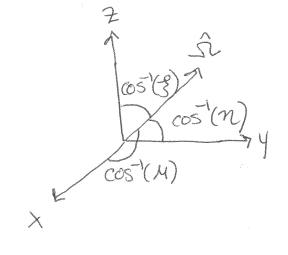
\includegraphics[keepaspectratio, width = 2 in]{../figs/cosines}
    \end{center}    
    \caption{Angle Space}
    \label{fig:angles}
\end{figure}
%
The streaming term is 
\begin{align*}
\vOmega \cdot \nabla \psi(\rvec, \vOmega, E) &= \mu \frac{\partial \psi}{\partial x} + \eta \frac{\partial \psi}{\partial x} + \xi \frac{\partial \psi}{\partial z} \\
\mu^2 &+ \eta^2 + \xi^2 = 1 \\
\vOmega &= \mu \hat{x} + \eta \hat{y} + \xi \hat{z}
\end{align*}
%
%Note that in this figure $\vOmega$ is a direction of motion of a point on a unit sphere, not a point in space.

We will use Figure~\ref{fig:stream} in our derivation, with $\vec{r} = \rvec_0 + s(\mu \hat{x} + \eta \hat{y} + \xi \hat{z})$, where $\rvec_0$ is an arbitrary point.
Further $x = x_0 + s\mu$, $y = y_0 + s\eta$, and $z = z_0 + s\xi$.
%
\begin{figure}[h!] 
    \begin{center}
    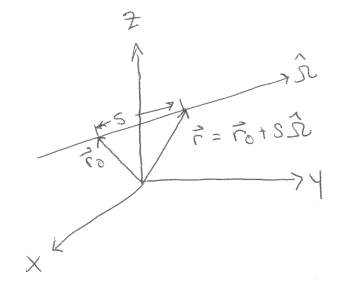
\includegraphics[keepaspectratio, width = 2.5 in]{../figs/moc-stream}    
    \end{center}   
    \caption{Characteristic Line}
    \label{fig:stream}
\end{figure}

Using this we can see
\[\frac{d\psi}{ds} = \frac{d\psi}{dx}\underbrace{\frac{dx}{ds}}_{\mu} + \frac{d\psi}{dy}\underbrace{\frac{dy}{ds}}_{\eta} + \frac{d\psi}{dz}\underbrace{\frac{dz}{ds}}_{\xi}\:,\]
which shows 
\[\frac{d\psi}{ds} = \vOmega \cdot \nabla \psi\:,\]
Now we can look at
\begin{equation}
\frac{d}{ds}\psi(\rvec_0 + \vOmega s, \vOmega, E) + \Sigma_t \psi = q(\rvec_0 + \vOmega s, \vOmega, E)\:.
\label{eq:ds-te}
\end{equation}
This is a derivative along a characteristic curve. 
The equation is a linear, first-order ODE that can be integrated. 


We will do this by introducing an integrating factor: $\exp[\int^s ds'' \: \Sigma_t(\rvec_0 + \vOmega s'', E)]$, which is the total number of points from an arbitrary starting point to the point $s$ distance away.

-----------\\
Note: if you are unfamiliar with integrating factors, look in a textbook or Wolfram Mathworld (when I first saw this material I hadn't learned about them and was pretty confused). \\
--------

First, we will note that
\[\frac{d}{ds}\exp[\int^s ds'' \: \Sigma_t(\rvec_0 + \vOmega s'', E)] = \exp[\int^s ds'' \: \Sigma_t(\rvec_0 + \vOmega s'', E)] \Sigma_t(\rvec_0 + \vOmega s, E)\]
And that
\begin{align*}
\frac{d}{ds}\bigl[\exp[\int^s ds'' \: \Sigma_t(\rvec_0 &+ \vOmega s'', E)]\psi(\rvec_0 + \vOmega s, \vOmega, E)\bigr] =\\ &\exp[\int^s ds'' \: \Sigma_t(\rvec_0 + \vOmega s'', E)]\frac{d \psi}{ds} + \psi \Sigma_t \exp[\int^s ds'' \: \Sigma_t(\rvec_0 + \vOmega s'', E)]
\end{align*}
We can see that the rhs of this expression is equal to the lhs of Eqn.~\ref{eq:ds-te} multiplied by the integrating factor.

We can therefore multiply the rhs of Eqn.~\ref{eq:ds-te} by the same factor and say:
%
\begin{equation}
\frac{d}{ds}\bigl[\exp[\int^s ds'' \: \Sigma_t(\rvec_0 + \vOmega s'', E)]\psi(\rvec_0 + \vOmega s, \vOmega, E)  \bigr] = \exp[\int^s ds'' \: \Sigma_t(\rvec_0 + \vOmega s'', E)]q(\rvec_0 + \vOmega s, \vOmega, E)
\label{eq:int-fact}
\end{equation}
%
Now, we will integrate this equation from $s'=-\infty$ to $s'=s$. Let's first look at the lhs of Eqn.~\ref{eq:int-fact}. 
%
\begin{align*}
\int_{-\infty}^s ds' \: \frac{d}{ds'}&\bigl[\exp[\int^{s'} ds'' \: \Sigma_t(\rvec_0 + \vOmega s'', E)]\psi(\rvec_0 + \vOmega s', \vOmega, E)  \bigr]  \\
= \: &\exp[\int^{s'} ds'' \: \Sigma_t(\rvec_0 + \vOmega s'', E)]\psi(\rvec_0 + \vOmega s', \vOmega, E)  |_{-\infty}^s  \\
= \: &\psi(\rvec_0 + \vOmega s, \vOmega, E) \exp[\int^{s} ds'' \: \Sigma_t(\rvec_0 + \vOmega s'', E)] \\
&- \psi(-\infty, \vOmega, E) \exp[\int^{-\infty} ds'' \: \Sigma_t(\rvec_0 + \vOmega s'', E)]
\end{align*}
The second term here goes to 0 since the integrating factor is going to 0 ($e^{-\infty} \rightarrow 0$). 

\begin{figure}[h!] 
    \begin{center}
    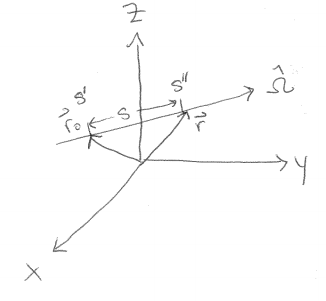
\includegraphics[keepaspectratio, width = 2.5 in]{../figs/moc-s}    
    \end{center}   
    \caption{Integration Lengths}
    \label{fig:int-s}
\end{figure}
%
Now, we can combine this with the rhs of Eqn.~\ref{eq:int-fact}:
\begin{align*}
\psi(\rvec_0 + \vOmega s, \vOmega, E) &\exp[\int^{s} ds'' \: \Sigma_t(\rvec_0 + \vOmega s'', E)] = \int_{-\infty}^s ds' \:\exp[\int^{s'} ds'' \: \Sigma_t(\rvec_0 + \vOmega s'', E)]q(\rvec_0 + \vOmega s', \vOmega, E) \\
%
&\psi(\rvec_0 + \vOmega s, \vOmega, E) = \int_{-\infty}^s ds' \:\exp[-\int_{s'}^s ds'' \: \Sigma_t(\rvec_0 + \vOmega s'', E)]q(\rvec_0 + \vOmega s', \vOmega, E)
\end{align*}
%
Functionally, this means that the flux at any point is a result of all sources up to that point attenuated by the exponent of the negative integral of the total number of mfps up to that point. See Figure~\ref{fig:int-s}.





\end{document}
